
\chapter{State of the Art}
\label{stateart}

Most of today’s programmers produce code and design applications using sequential programming paradigms. The application behaviour is designed and tested only for sequential execution, where the only parallelism is performed by the compiler at the instruction level, or by the hardware through the use of superscalarity and out-of-order execution. A few years ago a transition from single core very fast CPUs to slightly slower multicore CPUs started to happen. Since it was not possible to make CPUs faster by increasing their clock frequency due to heat dissipation problems, manufacturers opted to include many CPUs (now designated as cores) in the same chip, interconnected and sharing the same memory space. Now, instead of producing faster CPUs, manufacturers focused on increasing their processing throughput. Unfortunately, these newer CPUs (now including many cores) need a different programming paradigm to get the most performance possible when designing an application; programmers training did not accompany this transition to parallel programming paradigms that take advantage of this increase in processing throughput.

Programming for multicore environments require some knowledge of the underlying architectural concepts. Shared memory, cache coherence and consistency and data races are architectural aspects that the programmer did not have to face in sequential execution environments. Now, when designing an application, all these aspects must be taken into account, not only to ensure efficient use of the computational resources, but also the correctness of the application.

Heterogeneous computer architectures are becoming increasingly popular. They combine the flexibility of multicore CPUs with the specific capabilities of many-core accelerator devices, connected by PCI-Express interfaces. However, most computational algorithms and applications are designed with the specific characteristics of CPUs in mind. Even multithreaded applications cannot be easily ported to these devices expecting high performance. To optimize the code for these specific devices it is necessary to deeply understand the architectural principles behind their design.

These devices are usually made from small processing units, designed to achieve the most performance possible on specific problem domains, as opposed to conventional CPUs. They are oriented for massive data parallelism processing (SIMD architectures), offloading the CPU from such data intensive operations. Several many-core accelerator devices are available, ranging from the general purpose GPUs, to the \intel Many Integrated Core line, currently known as \intel Xeon Phi \cite{Intel:MIC}, and Digital Signal Processors (DSP) \cite{Texas:DSP}. An heterogeneous platform may have one or more accelerator devices of the same or different types.

Many libraries and development frameworks were already developed for these new heterogeneous platforms. They range from frameworks to abstract the inherent complexity of these systems, such as OpenACC \cite{OpenACC} or GAMA \cite{GAMA}, to specialized high performance libraries for some specific scientific domains, such as CuBLAS \cite{NVIDIA:CuBLAS}.

A more in-depth analysis of these two groups of state of the art technology (hardware and software) will be presented in the next sections.

\section{Hardware Environment}

Different accelerator devices opt to use distinct approaches to solve their domain specific problems, leading to small, but important, architectural differences. If these details are not taken into account, it may not be possible to make efficient code, underusing the specialized resources of these devices.

The Single Instruction Multiple Data (SIMD) parallelism model is common ground for most accelerator devices architectures. It is designed to get the most throughput when processing information by applying the same instruction, in parallel, to large sets of independent data. SIMD processors originated in 1970, designated as vector supercomputers, and was popularized by Cray. However, these supercomputers were too specialized for most common processing needs. The current CPUs are including some of the characteristics of vector processors, such as the creation of SSE, and later AVX, instructions from \intel. These extensions to their x86 instruction set, and new special registers capable of holding up to 256 bits (AVX), are extremelly useful for processing highly data parallel algorithms. Current accelerator devices adopted this model in their architectures, as it fits to the needs of the specific problems that they were developed for, such as the GPUs.

Consider GPUs and image processing as an example to justify the use of the SIMD model. Each pixel that is rendered is independent from all other pixels on the image. Their computation result from the same instructions but on different independent data, thus making their processing embarrassingly parallel. For achieving maximum performance, one important characteristic of the code, common to most accelerator device architectures, is that it needs to explore the most parallelism possible between the data to be processed, also known as data parallelism. Other device specific properties, with interest for the programmer, will be discussed later.

Load balancing is always a challenge when programming for parallel environments. Even when using only multicore CPUs, it is important to manage how much load each core is processing, so that every core is working most of the time. If the workload is badly distributed, there will be cores stalled waiting for others to complete, wasting the available computational resources. However, it also depends on the nature of the problem; regular problems are easier to balance than irregular problems, which usually require a dynamic load balancing strategy at runtime, since the execution time of the parallel tasks is not predictable. The same concept also aplies to the dataset: it has to be properly distributed among the available resources in such a way that the CPU and devices take the roughly the same time to process.

Heterogeneous architectures open the possibility of running parallel tasks on both CPU and accelerators simultaneously. However, due to their technical differences, the same task can take different amount of time to complete depending in where it is executed. This creates another layer of complexity when dealing with the workload balance. Now, while managing the workload distribution inside the CPU (between its cores), and also inside the accelerator device chip (with a mechanism similar to the CPU), it is also relevant to manage the distribution between CPU and accelerator device. It is important to have a good control over the load balancing, specially in these hybrid systems, in such a way that neither of the processing units (CPU and accelerator devices) becomes stalled waiting for the other to complete, and thus not wasting any computational resources. Also, the load balancing must be done with the least communication possible between CPU and accelerator, since the time it takes to complete is usually high.

As of 2012, over 50 of the TOP500’s list \cite{TOP500} are powered by GPUs, which indicates an exponential growth in usage when compared to previous years. The \intel Xeon Phi is also becoming popular, being the accelerator device of choice in 7 clusters of the TOP500.

\subsection{The GPU as Computing Accelerator}

There are several accelerator devices currently arriving, or already, on the market. The first and most common are General Purpose Graphics Processing Units (GPGPUs). Recently, GPGPU makers allowed drivers to execute code that is not produced for image rendering. However, there are specific hardware details that were designed only for image rendering purposes, which limit the utilization of these devices for certain types of algorithms. One example was the use of only single precision float point arithmetic in the early GPGPUs design.

This type of devices are specialized for massive data parallelism, where the same instruction is simultaneously applied to large amounts of data. One example of a problem domain that can take advantage of these characteristics is the multiplication of matrices, which is very common in scientific applications. As GPGPUs evolved, the support for specific scientific demands was added, such as support for double precision float point arithmetic and compliance to all IEEE float point arithmetic rules.

Recently, \nvidia \cite{NVIDIA} launched a line of GPUs designed for scientific computation rather than image processing \cite{NVIDIA:Tesla}. This category of devices, known as the Tesla, has more GDDR RAM, processing units and a slight different design suitable for use in cluster computational nodes (in terms of size and cooling). The chip has suffered some changes too, increasing the cache and the amount of processing units. In this dissertation two different \nvidia GPUs will be used, the \nvidia Tesla C2070 (Fermi architecture \cite{NVIDIA:Fermi}) and the new \nvidia Tesla based on the GK110 chip (Kepler architecture \cite{NVIDIA:Kepler}).

The \nvidia GPUs architecture has two main components: computing units (Streaming Multiprocessors, known as SM) and the memory hierarchy (global external memory, GDDR5 RAM, and 2-level cache and shared memory block). Each SM contains a set of \cuda cores, which are processing units that perform both integer and float point arithmetic (additions, multiplications and divisions). These SMs also have some specialized processing units for only square roots, sins and cosines, as well as a warp scheduler (warps will be explained later) to match \cuda threads to \cuda cores, load and store units, register files and the L1 cache/shared memory.

\nvidia considers that a parallel task is constituted by a set of \cuda threads, which will execute the same instructions (conditional jumps are a special case that will be explained next) but on different data. This set of instructions is considered a \cuda kernel, in which the programmer defines the behavior of the \cuda threads. A simple way to visualize this concept is by considering the example of multiplying a scalar with a matrix. In this case, a single thread will handle the multiplication of the scalar by an element of the matrix, and it is needed to use as many \cuda threads as matrix elements.

The \cuda threads are organized in a hierarchy. A block is a set of \cuda threads that is matched by the global scheduler to run on a specific SM. A grid is a set of blocks, representing the whole parallel task. Considering the scalar-matrix multiplication example, each \cuda thread calculates the value of an element of the matrix, and they are organized in blocks, which can represent all the calculations for a single line of the matrix. The grid holds all the blocks responsible for calculating all the new values of the matrix. Note that both the block and the grid have a limited size.

A warp is a set of \cuda threads (in both Fermi and Kepler architectures it has a size of 32 \cuda threads), scheduled by the SM scheduler to run on its SM at a given time. A warp can only be constituted by \cuda threads from the same block.

When programming these devices, conditional jumps must be avoided at all costs if they lead to divergence of the \cuda threads within the same warp. Within an SM it is not possible to have 2 threads executing different instructions at the same time. So, if there is a divergence between the threads within the warp, the two conditional branches will be executed one after the other, doubling the warp execution time. The high latency of accessing the GPU memory os another important detail to take into account. To hide this latency, and avoid the GPU of becoming stalled, the strategy behind the \nvidia architectures is to provide the GPU with the most number of \cuda threads possible. This allows the schedulers to keep a scoreboard of which warps are ready to execute and which are waiting for data to load, hopefully never starving the \cuda cores.

Since the GPU is connected by PCI-Express interface, the bandwidth for communications between CPU and GPU is restricted to only 12 GB/s (6 GB in each direction of the communication). Memory transfers between the CPU and GPU must be minimal as it greatly restricts the performance.

Architecture specific details, relevant to the programmer, of both Fermi and Kepler will be presented in the next subsections.

\subsubsection{\nvidia Fermi Architecture}

The relevant architectural details of this architecture, specifically for the Tesla C2070, are explained in this section. The Fermi architecture is schematized in figure \ref{fig:fermi}.

\begin{figure}[!htp]
	\begin{center}
		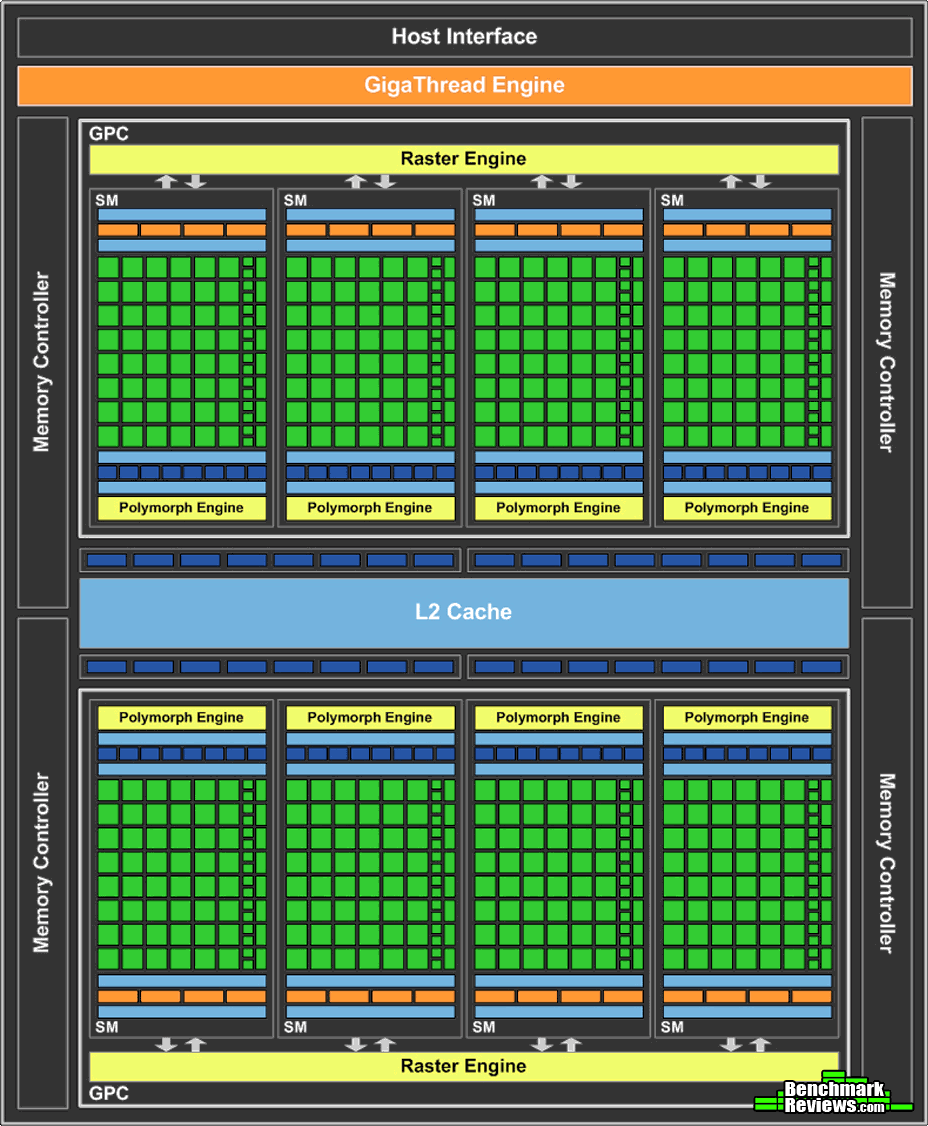
\includegraphics[scale=0.25]{../../common/img/fermi_arch.png}
		\caption{Schematic representation of the \nvidia Fermi architecure.}
		\label{fig:fermi}
	\end{center}
\end{figure}

In the Tesla C2070, each SM has 32 \cuda cores, with 14 SM per chip, making a total of 448 \cuda cores. Theoretically, it is possible to have 448 \cuda threads running at the same time. In each SM there are 4 Special Functional Units (SFU) to process special operations such as square roots and trignometric arithmetic.

Memory wise, these devices have a slightly different memory hierarchy than the CPUs, but still with the faster and smaller memory closer to the \cuda cores. Each \cuda thread can have up to 63 registers, but when large amounts of threads are used this amount diminishes, which can, in some cases, lead to register spilling (when there is not enough registers to hold the variables values and they must be stored in local memory, which is the external RAM).

Within a SM there is a block of configurable 64 KB memory. In this architecture it is possible to use it as 16 KB for L1 cache and 48 KB for shared memory, or vice-versa (only shared between threads of the same block). The best configuration is dependent of the specific characteristics of each algorithm, and usually requires some preliminary tests to evaluate which configuration obtains the best performance. Shared memory can also be used to hold common resources to the threads, even if they are read-only, avoiding accesses to the slower global memory.

The L2 cache is slower but larger, with the size of 768 KB. It is shared among all SMs, opposed to the L1 cache. The global memory is the last level of on device memory. The Tesla C2070 has a total of 6 GB GDDR5 RAM, with a bandwidth of 192.4 GB/s.

One important detail for efficient memory usage is to perform coalesced memory accesses. Since the load units get memory in blocks of 128 bits, it is possible to reduce the amount of loads by guaranteeing that all threads that need to load data, preferably if it is continuous on the address space (such as contiguous elements of an array), do it at the same time. This allows the memory controller to find the best grouping of thread loads and consolidates them in fewer memory accesses \cite{NVIDIA:Fermi}.

Finally, on the Fermi architecture it is only possible to run one kernel at a time on the GPU.

\subsubsection{\nvidia Kepler Architecture}

The Kepler and Fermi architectures have many similarities so only the relevant differentiating aspects will be presented.

The Streaming Multiprocessor present in the Fermi architecture was changed to hold more, but smaller, \cuda cores (now 192), working at half the speed of the previous \cuda cores, since the shader clock was removed. The individual performance of the \cuda cores is lower but the overall performance of the GPU has increased. These new Streaming Multiprocessors are now known as SMX and it is possible to have up to 2880 \cuda cores in only one chip. The schematic representation of the Kepler architecture is presented in figure \ref{fig:kepler}.

The maximum amount of registers per \cuda thread was increased from 63 to 255. A new read-only cache of 48 KB was added at the same hierarchy level of the L1 cache. The size of the L1/shared memory block is the same as Fermi, but adds a new configuration of 32/32 KB for each type. The L2 cache size has increased to 1536 KB, and its hit bandwidth is 73\% larger than on Fermi.

\begin{figure}[!htp]
	\begin{center}
		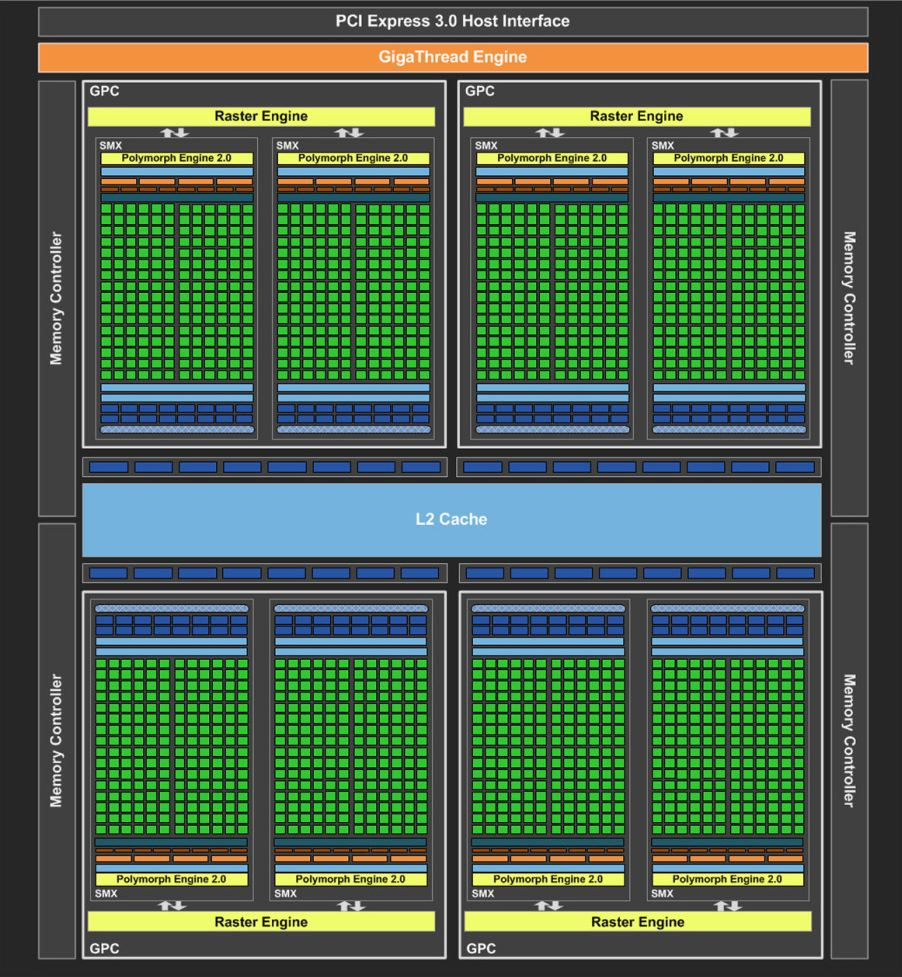
\includegraphics[scale=0.4]{../../common/img/kepler_arch.jpg}
		\caption{Schematic representation of the \nvidia Kepler architecture.}
		\label{fig:kepler}
	\end{center}
\end{figure}

Programming-wise, a set of new important features has been added to this architecture. One of them is the Dynamic Parallelism. Now it is possible to \cuda threads spawn other threads, without it being explicitly required by the host (CPU). It allows for improvements in irregular problems, such as Monte Carlo ray tracing. Another feature is the Hyper-Q, which allows multiple cores of the same CPU to use and spawn kernels on the same GPU. Also, it is now possible to run several different kernels in the same GPU at the same time, where they will be scheduled to different SMX. Finally, a new shuffle instruction has been added to the instruction set. By using this instruction, \cuda threads can now read values directly from each other, within the same warp, without the need of using shared memory.

The problem of coalesced memory accesses is still present. However, while Fermi load units get blocks of 128 bits, load units on the Kepler architecture are capable of getting blocks of 256 bits \cite{NVIDIA:Kepler}.

\subsection{The \intel Many Integrated Core architecture}

The \intel Many Integrated Core (MIC architecture), currently known as \intel Xeon Phi, has a different conceptual design than the Nvidia GPUs. A chip can have up to 61 multithread cores, with 4 threads per core, and it is more focused on vectorization \cite{Intel:MIC:Elgar}. 

\begin{figure}[!htp]
	\begin{center}
		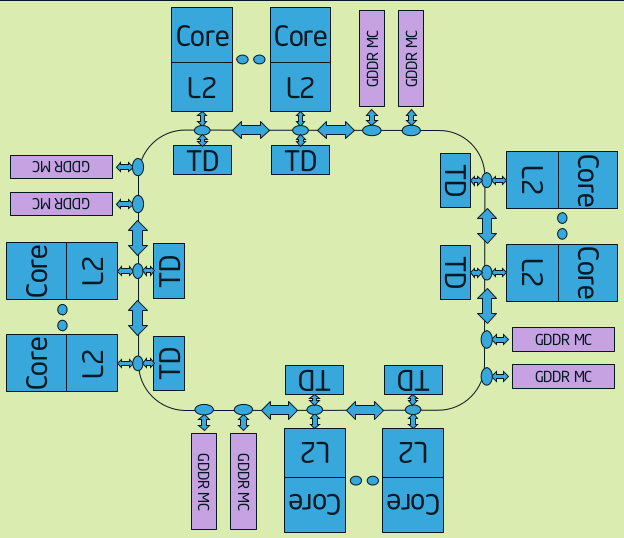
\includegraphics[scale=0.5]{../../common/img/mic_arch.png}
		\caption{Schematic representation of the \intel MIC architecture.}
		\label{fig:mic}
	\end{center}
\end{figure}

It has 32 512 bit wide vector registers per core, with the capacity of holding 16 single precision float point values. The L2 cache size is 512 KB per core and the chip comes with 6 to 8 GB of GDDR5 RAM, providing up to 320 GB/s of throughput. It was designed for memory bound problems, as opposed to GPUs (Fermi only has a bandwidth of 192.4 GB/s), but Intel will also launch a different version of the chip tuned for compute bound problems.

Unlike conventional CPUs, the MIC cores do not share any cache, therefore cache consistency and coherence is not assured. If needed, data must be explicitly passed between cores, as in a distributed memory system. The cores are connected in a ring network, as represented in figure \ref{fig:mic}.

The MIC uses the same instruction set as conventional x86 CPUs. This allows to easily port current libraries to run on this device. Furthermore, Intel has already announced that a tuned MPI library will be available for this device.

\section{Development Frameworks}

Application development for homogeneous systems with multicore CPUs has been around for some time. There are some libraries that attempt to abstract the programmer from specific architectural and implementation details, providing an easy API as close as possible to current sequential programming paradigms.

Developing applications for heterogeneous systems, with both CPU and accelerator devices, poses a series of new challenges due to the change of programming paradigm. However, some frameworks attempt to abstract the inherent complexity of these platforms.

Frameworks that attempt to ease the programmer’s job, while providing scalable and flexible solutions will be presented through the next subsections. Other frameworks that will not be used are not presented.

\subsection{OpenMP}

For shared memory systems, where there is one or more multicore CPUs sharing the same memory address space, one of the most popular libraries for task parallelization is OpenMP \cite{OpenMP}. This API is designed for multi-platform shared memory parallel programming in C, C++ and Fortran, on all available CPU architectures. It is portable and scalable, aiming to provide a simple and flexible interface for developing parallel applications, even for the most inexperienced programmers.

While being simple to use, OpenMP allows experienced users to fine-tune the code, providing various task schedulers, as well as instructions for controlling more efficiently the shared memory accesses and parallel execution of the tasks.

\subsection{OpenACC}

OpenACC \cite{OpenACC} is a framework for heterogeneous platforms with accelerator devices. It is designed to simplify the programing paradigm for CPU/GPU systems by abstracting the memory management, kernel creation and GPU management. Like OpenMP, it is designed for C, C++ and Fortran, but allowing the parallel task to run on both CPU and GPU at the same time.

While it was originally designed only for CPU/GPU systems, they are currently working on the support for the new Intel Xeon Phi \cite{OpenACC:HPCWire}. Also, they are working alongside with the members of OpenMP to create a new specification supporting accelerator devices in future OpenMP releases \cite{OpenACC:OpenMP}.

\subsection{GAMA}

The GAMA framework \cite{GAMA} has the same purpose of OpenACC, of providing the tools to help building efficient and scalable applications for heterogeneous platforms, but opts for a different strategy. It aims to create an abstraction layer between the architectural details of heterogeneous platforms and the programmer, aiding the development of portable and scalable parallel applications. However, unlike OpenACC, its main focus is on obtaining the best performance possible, rather than abstracting the architecture from the programmer. The programmer to still needs to have some knowledge of each different architecture, and it is necessary to instruct the framework about how tasks should be divided, in order to fit the requirements of the different devices.

The framework frees the programmer from managing the workload distribution (apart from the dataset division), memory usage and data transfers between the available devices. However, it is possible for the programmer to tune these specific details, if he is confortable enough with the framework.

GAMA assumes a hierarchy composed of multiple devices (both CPUs and GPUs, in its terminology), where each device has access to a private address space (shared within that device), and a distributed memory system between devices. To abstract this distributed memory model, the framework offers a global address space. However, since the communication between different devices is expensive, GAMA uses a relaxed memory consistency model, where the programmer can use a synchronization primitve to enforce memory consistency.

\subsection{Debugging}

Debugging applications in shared memory systems is a complex task, as the errors are usually harder to replicate than on sequential applications. Bugs can happen due to deadlocks, unexpected changes to the shared memory, data inconsistency and incoherence. While there are some tools to efficiently debug sequential applications, such as the GNU Debugger \cite{GDB}, they lack on the support for multithreaded applications. Unfortunately, there are no debuggers that can efficiently be used to debug a parallel application.

The effort necessary to debug these applications, without the use of any third-party tools, is directly related to the programmers experience and knowledge of working with shared memory systems. However, even the most experienced will face complex obstacles when debugging for more than 4 threads, as the application behavior is much harder to control.

Nvidia offers a tool for debugging \cuda kernels on their GPUs, which is based on the GNU Debugger \cite{NVIDIA:gdb}. It is useful when used to find bugs in the kernels, but only in the same way that a sequential application is debugged. Also, when using more than 2-4 \cuda threads it does not help the programmer at all, considering that \cuda kernels can reach to the thousands of threads.

\newpage
